\documentclass[a4paper,11pt,uplatex]{jsbook}
%\usepackage{fancyhdr}
\setlength{\footskip}{16pt}
\usepackage{amsmath}
\usepackage[dvipdfmx]{graphicx}
\usepackage[dvipdfmx]{color}
%\usepackage{pagecolor}[white]
\usepackage{amsmath,amssymb}
%\usepackage[top=3cm, bottom=3cm, left=3cm, right=3cm]{geometry}
\usepackage{braket}
\usepackage{bm}
\numberwithin{equation}{section}
\usepackage{mathrsfs}
\usepackage{siunitx}
\usepackage{physics}
\usepackage[dvipdfmx]{graphicx}
\usepackage[compat=1.1.0]{tikz-feynhand}
\usepackage{caption}
\usepackage{subcaption}
%\usepackage{cleveref}
\usepackage{float}
\usepackage{multicol}
\setlength{\columnsep}{15mm}
%\usepackage[style=phys,articletitle=false,biblabel=brackets,chaptertitle=false,pageranges=false]{biblatex}
%\usepackage[style=phys]{biblatex}
\usepackage[dvipdfmx]{hyperref}
\usepackage{url}
\usepackage{pxjahyper}
\usepackage{bookmark}
%\usepackage[backref]{hyperref}
\setcounter{tocdepth}{3}
\setlength{\parindent}{2em}
\def\vector#1{\mbox{\boldmath $#1$}}
\def\slash#1{\not\!#1}
\def\slashb#1{\not\!\!#1}
\def\delsla{\not\!\partial}
%\usepackage[dvipdfmx]{xcolor}


\hypersetup{
 setpagesize=false,
 bookmarksnumbered=true,%
 bookmarksopen=true,%
 colorlinks=true,%
 linkcolor=black,
 citecolor=red,
 urlcolor=black,
}
%backreferenceのカスタマイズ. "Back to p.3"のように表示する.
%\renewcommand*{\backref}[1]{(p.#1へ戻る)}
%\newcommand{\backtoc}{\hyperlink{toc}{[目次へ]}}
\newcommand{\backtoc}{\texorpdfstring{\protect\hyperlink{toc}{\hspace{5pt} \scriptsize [目次へ]}}{}}
\newcommand{\mychapter}[1]{\chapter[#1]{#1\backtoc}}
\newcommand{\mysection}[1]{\section[#1]{#1\backtoc}}
\newcommand{\mysubsection}[1]{\subsection[#1]{#1\backtoc}}

% 数式
%\usepackage{amsmath,amsfonts}
%\usepackage{bm}
%\usepackage{physics}
% 画像
%\usepackage[dvipdfmx]{graphicx}
%\usepackage[dvipdfmx,colorlinks=true,linkcolor=blue]{hyperref}
%\usepackage{pxjahyper}

\begin{document}


\chapter{MAMIにおける測定手法}
この章の目的は、実験に用いた装置の性能や仕様、およびセットアップの手法を説明することである。
また、データ取得の手順を示す。
\section{装置とセットアップ}
\subsection{マインツマイクロトロン(MAMI)}
Mainz Microtron(MAMI)はドイツ、マインツ大学が所有する連続電子線加速器施設である。最大エネルギー1508 MeVの電子ビームを供給する
3台のRTM(Race Track Microtron)および1台のHDSM(Harmonic Double Siided Micrtron)から構成される。
ハイパー核生成実験ではHDSMを用いて最大エネルギーの1508 MeVの電子ビームを供給する。
スペクトロメータ較正実験では、RTM3までで加速された180 MeVから210 MeVまでの電子ビームを用いる。
RTM3ではストリップによる加速の回数によって15 MeV間隔でエネルギーを変えることができる。
今回、崩壊パイ中間子法で放出される$\pi$中間子はおよそ130 MeVであり、理想的には同じ運動量の散乱電子によってスペクトロメータ較正を
行うことが望ましい。しかしながらMAMIの供給可能な最低エネルギーは180 MeVであるため、この領域の電子ビームを用いて外挿する形で較正を行っている。
\begin{table}
  \begin{tabular}{cc}
    \hline
    RTM3 & 180 MeV - 210 MeV \\
    HDSM & 1508 MeV \\
    \hline
  \end{tabular}
\end{table}

\subsubsection{電子ビームライン}
200 MeV領域の電子ビームはX1ビームラインに供給される。
以下にX1ビームラインの構成を示す。
ビーム調整を行うsteere電磁石はRTM3に設置されている。
四重極磁石が配置されている。
アンジュレータとビームダンプが配置されている。


\subsubsection{ビーム調整}
まずビームプロファイルモニタを用いてフェイントビームの位置を目測で調整する。この時の精度は数 mm 程度である。
続いて、ビーム強度を5 $\mu\text{A}$に上げつつ放射線レベルが基準値よりも低くなるように微調整を行う。
この時放射線レベルが安全基準よりも高くなることは、ビームがビームダンプまで輸送されるまでにビームパイプ中心から外れていることを示す。
最後にカメラを用いて放射光を見ながらビームの位置を調整する。スリットに対してビーム中心がずれている場合には回折パターンが上下非対称になる。

\subsection{アンジュレータ}
\subsubsection{磁場制御}
マトリックス型のホールプローブを用いて磁場を測定する。
隣り合う電磁石の磁場が影響するため、適切な磁場を得るためには全ての電磁石の電流を同時に調整する必要がある。
そのため、測定と電流のチューニングを繰り返し行う。
アンジュレータ通過後の電子ビームの方向のずれを最小に抑えることが重要となる。

\subsubsection{位置制御と読み取り}
位置制御はモータで行う。可動範囲は 825 mm、間隔は 5 mmで指定する。
移動したアンジュレータの絶対値は、リニアエンコーダ(Heidenhain LC415)で 5 $\mu m$ の精度で読み出すことができる。
\subsubsection{アラインメント}
セオドライトを用いてビームライン中心とアンジュレータ中心
\subsection{分光光学系}
\subsubsection{スリット}
\subsubsection{grating}
\begin{itemize}
  \item フーリエ変換
  \item 分光
\end{itemize}

\subsubsection{波長分散レンズ}
\begin{figure}[tb]
  \centering
  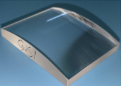
\includegraphics[width=0.8\linewidth]{image/3-lens.png}\\
  \caption{レンズ}
  \label{lens}
\end{figure}
\subsubsection{CMOS カメラ}
光学系は波長が400 nmの領域において働くため、可視光領域のカメラを用いることができる。HAMAMATSU C14440-20UPを用いた。
仕様を
\begin{table}[h]
\centering
\begin{tabular}{c|c}
  ピクセル数 & 2304 $\times$ 2304\\
  ピクセルサイズ & 6.5 $\mu$m $\times$ 6.5 $\mu$m\\
  チップサイズ & 14.976 mm $\times$ 14.976 mm\\
  ビット深さ & 16 bit\\ 
\end{tabular}
\end{table}

\subsection{光学系のアラインメント}
青色レーザを用いて光軸中心が光学素子の中心を通るようにアラインメントを行う。

\section{データ取得}


\subsection{分光光学系の波長較正}
波長較正として水銀灯を用いる。
$400 \text{nm}$領域には2本の輝線があり、このスペクトルを光学系で観測することで2つの輝線スペクトルを観測できる。\\
水銀灯ランプはビームラインから垂直に5 mの位置に設置されており、ミラーを用いて電子ビームラインと同じ軌道を通って光学系に導かれる。\\

輝線スペクトルをガウス関数でフィッティングし、中心位置のピクセルを対応する波長にする。
2本のスペクトル以外のピクセルは2本の輝線の波長 -ピクセル関係の線形性を仮定して決定する。
\subsection{データ取得}
\begin{itemize}
  \item 指定の位置にアンジュレータが移動する
  \item カメラによる画像撮影の信号が4回送られる
  \item 画像撮影が完了するとDAQに信号が送られる
  \item アンジュレータのモータに次の指定位置の信号が送られる
  \item アンジュレータが指定位置まで移動する。
\end{itemize}
\subsubsection{配線}

\subsection{電子ビームエネルギー測定}

ビームラインの切り替え\\
プロファイルモニタによるビームチューニング\\
画像によるビームチューニング\\

\subsection{弾性散乱実験との同時運用}
弾性散乱実験と並行してアンジュレータによる電子ビームエネルギー測定を行った。
\subsection{下流側アンジュレータによるデータ測定}
パラメータ較正を目的として、下流側アンジュレータのみを用いたデータ取得を行う。


\end{document}